%!TEX root = ../Thesis.tex
\chapter{State Input Analysis}


\section{Analysing Objective}
\label{sec:state_input_objective}

The purpose of the state-input analysis is to investigate how the optimal
decision variables change as a function of the system state.

For a two-state system, the initial state is written as

\begin{equation}
    x_0 =
    \begin{bmatrix}
        x_1 \\
        x_2
    \end{bmatrix}
\end{equation}

A rectangular grid is constructed over the \((x_1,x_2)\) state plane. At
each grid point, the corresponding optimization problem is solved using that
state as the initial condition.

For the linear case, the analysis records the first optimal control input,

\begin{equation}
    u_0^\ast
    =
    f(x_1,x_2)
\end{equation}

For the bilinear case, both the first optimal control input and the first
optimal bilinear parameter are recorded,

\begin{align}
    u_0^\ast
    &=
    f(x_1,x_2)\\
    v_0^\ast
    &=
    g(x_1,x_2)
\end{align}

Only the first optimized values are considered because they represent the
immediate control decision associated with a particular state.

The state space is sampled over predefined intervals,

\begin{equation}
    x_1 \in
    [x_{1,\min},x_{1,\max}],
    \qquad
    x_2 \in
    [x_{2,\min},x_{2,\max}]
\end{equation}

and the optimization problem is solved independently for every point in this
grid.

The resulting values form surfaces over the state plane:

\begin{equation}
    (x_1,x_2)
    \longrightarrow
    u_0^\ast
\end{equation}

and, for the bilinear system,

\begin{equation}
    (x_1,x_2)
    \longrightarrow
    v_0^\ast
\end{equation}

These mappings provide a direct visualization of how the optimal decision
changes depending on the location of the system in the state space.

The surfaces are represented using both three-dimensional surface plots and
two-dimensional contour plots. The main objective of this analysis is therefore not to study a particular
trajectory, but to characterize the state-dependent structure of the
optimization problem. In particular, the plots make it possible to identify
regions in the state space where the optimal input changes gradually, changes
rapidly, approaches its bounds, or exhibits nonlinear behavior.

For the bilinear system, separate plots are produced for \(u_0^\ast\) and
\(v_0^\ast\). This allows the influence of the state on the two optimization
variables to be examined independently.


\section{Results}
\label{sec:state_input_results}

The state-input relation was evaluated using the stochastic bilinear system

\begin{equation}
    A(v)
    =
    A_{\mathrm{base}}
    +
    vA_v
\end{equation}

with

\begin{equation}
    A_{\mathrm{base}}
    =
    \begin{bmatrix}
        0.90 & 0 \\
        0 & 0.50
    \end{bmatrix}
\end{equation}

and

\begin{equation}
    A_v
    =
    \begin{bmatrix}
        0 & 1 \\
        0 & 0
    \end{bmatrix}
\end{equation}

Therefore,

\begin{equation}
    A(v)
    =
    \begin{bmatrix}
        0.90 & v \\
        0 & 0.50
    \end{bmatrix}
\end{equation}

The input and output matrices were

\begin{equation}
    B
    =
    \begin{bmatrix}
        0 \\
        1
    \end{bmatrix},
    \qquad
    C
    =
    \begin{bmatrix}
        1 & 0
    \end{bmatrix}
\end{equation}

The prediction horizon was selected as

\begin{equation}
    N=15
\end{equation}

with weighting matrices

\begin{equation}
    Q=1,
    \qquad
    R_U=0.1,
    \qquad
    R_V=0.1
\end{equation}

The state-input relation was evaluated over

\begin{equation}
    -10
    \leq
    x_1
    \leq
    10,
    \qquad
    -10
    \leq
    x_2
    \leq
    10
\end{equation}

using a \(50\times50\) grid.

\subsection{Optimal Control Input Relation}

For every point in the \((x_1,x_2)\) grid, the nonlinear optimization
problem was solved and the first optimal control input \(u_0^\ast\) was
recorded.

The resulting surface represents

\begin{equation}
    u_0^\ast=f(x_1,x_2)
\end{equation}

\begin{figure}[H]
    \centering
    \begin{minipage}[t]{0.49\textwidth}
        \centering
        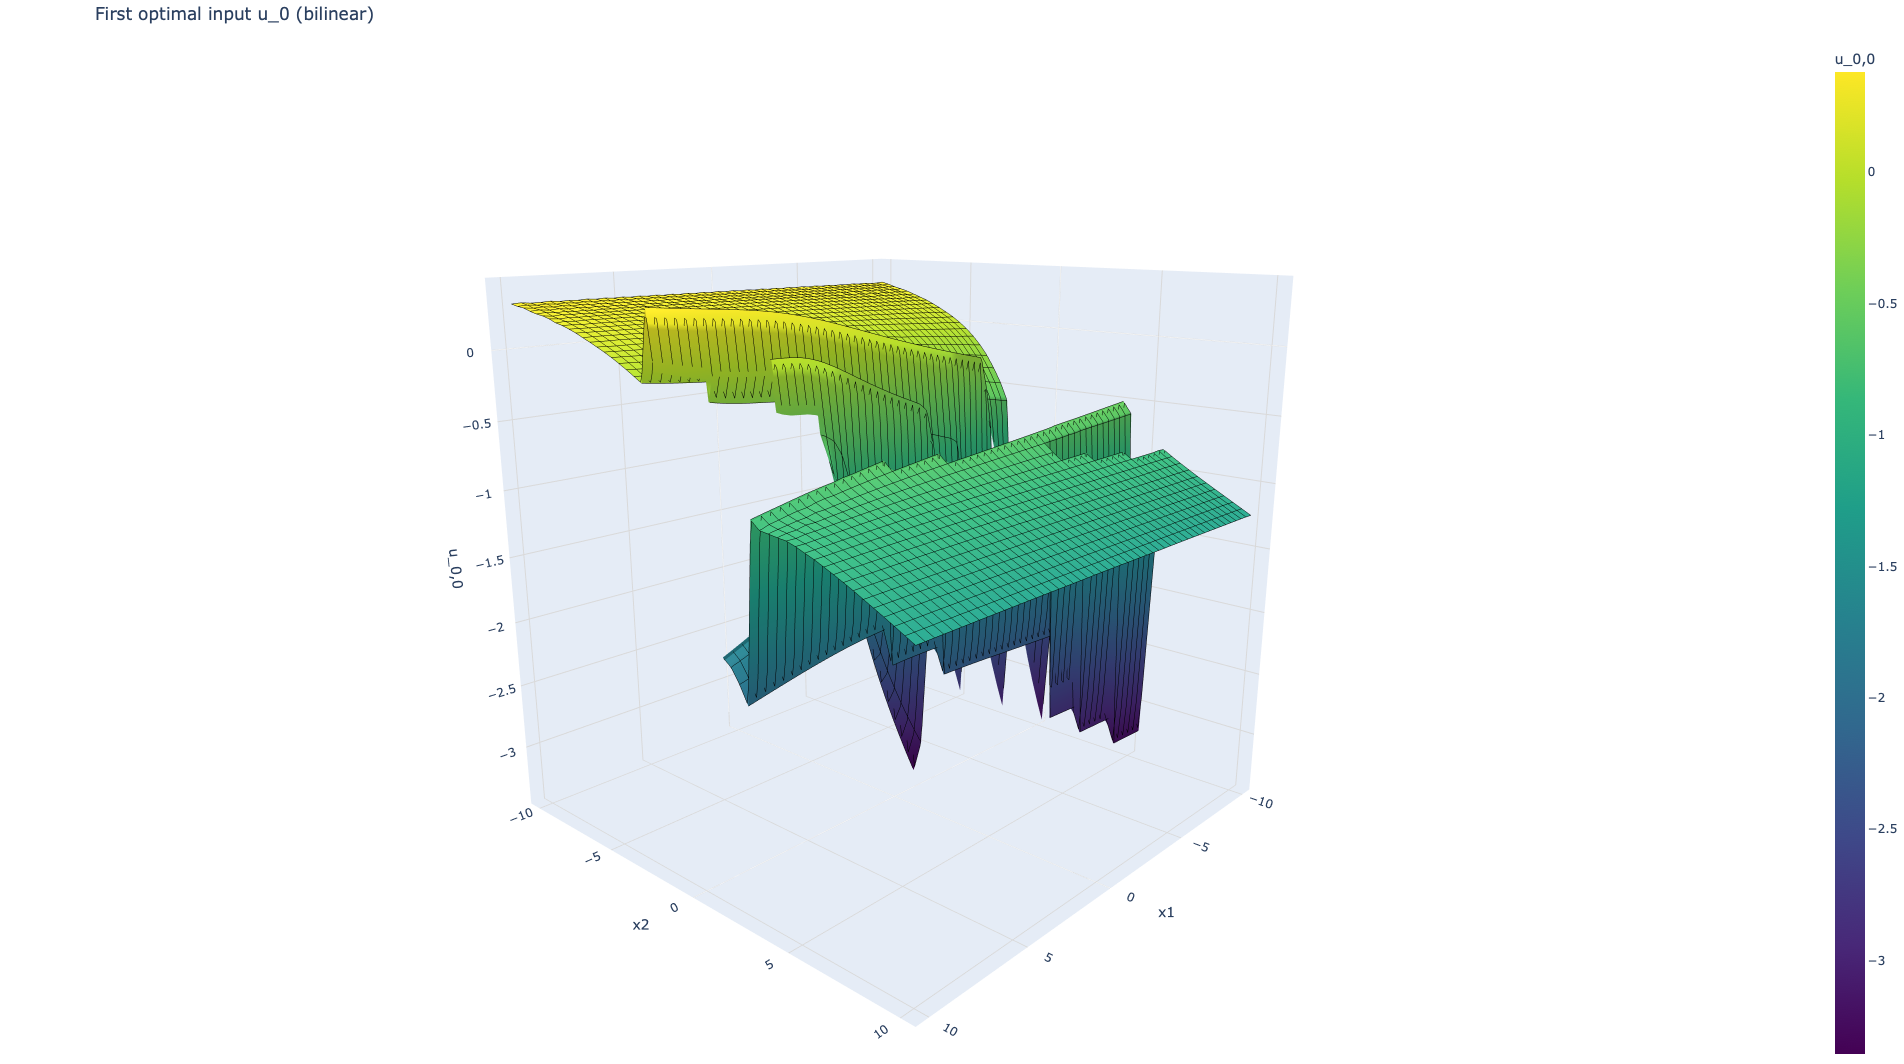
\includegraphics[width=\linewidth]{graphics/state_input_u_surface.png}
        \caption{First optimal control input \(u_0^\ast\) as a function of the
        initial state \((x_1,x_2)\)}
        \label{fig:state_input_u_surface}
    \end{minipage}
    \hfill
    \begin{minipage}[t]{0.49\textwidth}
        \centering
        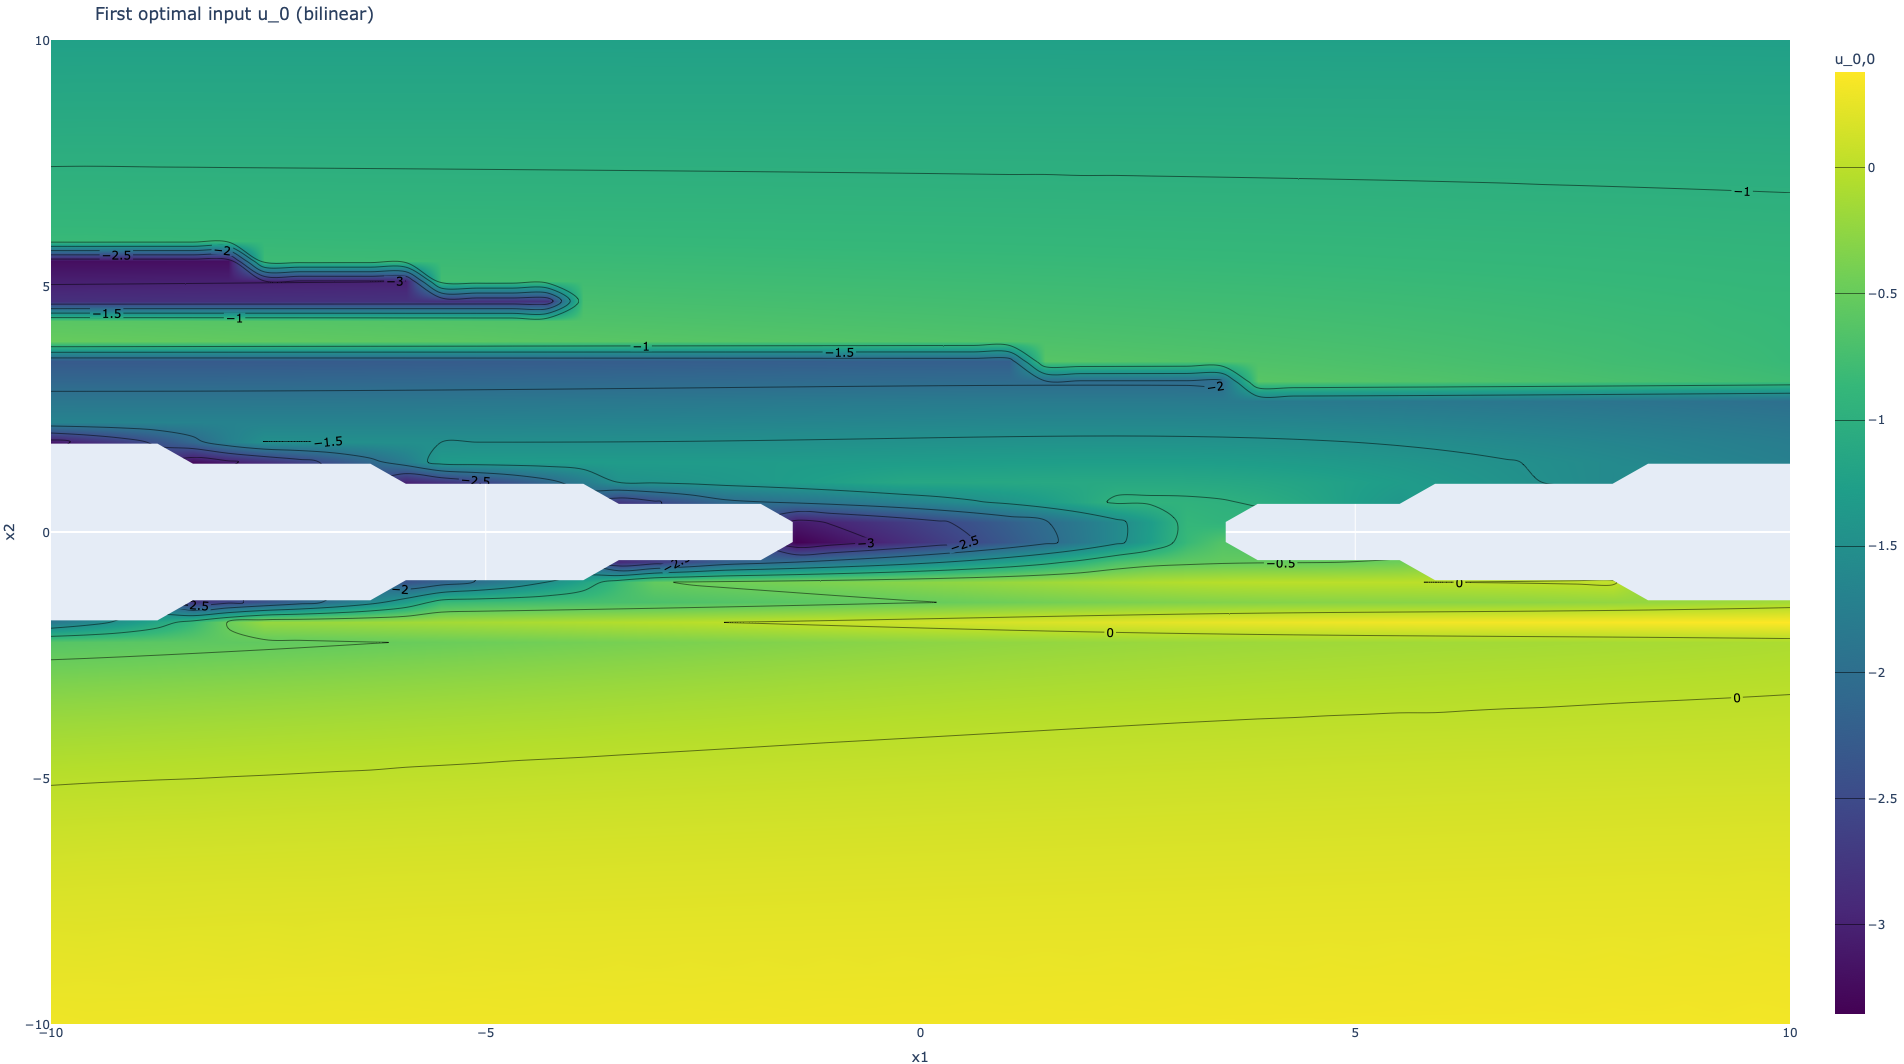
\includegraphics[width=\linewidth]{graphics/state_input_u_contour.png}
        \caption{Contour representation of \(u_0^\ast\) over the initial-state
        plane}
        \label{fig:state_input_u_contour}
    \end{minipage}
\end{figure}

The same relation is shown as a contour plot in
\cref{fig:state_input_u_contour}. The contour representation provides a
two-dimensional view of regions in the state space associated with similar
optimal control actions.



\subsection{Optimal Bilinear Parameter Relation}

The same state-space sweep was also used to evaluate the first optimal
bilinear parameter. For each initial state, the optimization therefore
provides

\begin{equation}
    v_0^\ast=g(x_1,x_2)
\end{equation}

\begin{figure}[H]
    \centering
    \begin{minipage}[t]{0.49\textwidth}
        \centering
        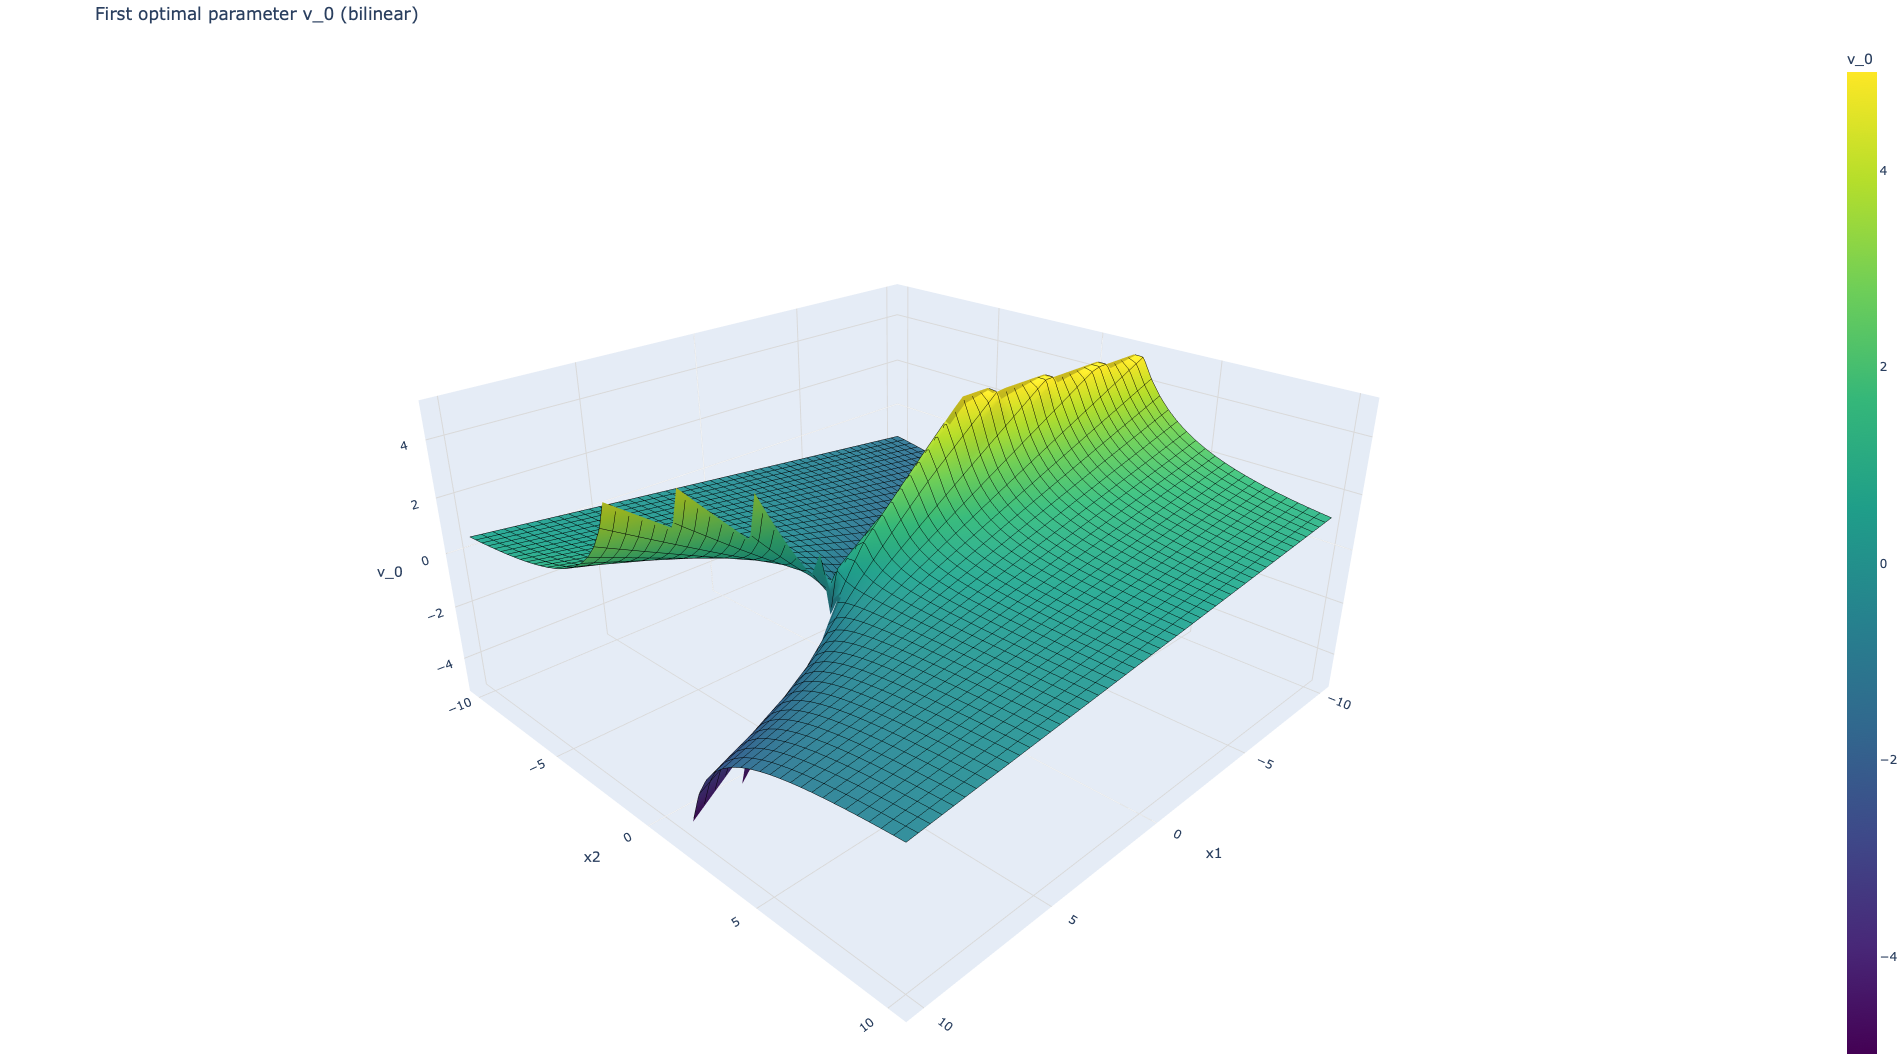
\includegraphics[width=\linewidth]{graphics/state_input_v_surface.png}
        \caption{First optimal bilinear parameter \(v_0^\ast\) as a function of
        the initial state \((x_1,x_2)\)}
        \label{fig:state_input_v_surface}
    \end{minipage}
    \hfill
    \begin{minipage}[t]{0.49\textwidth}
        \centering
        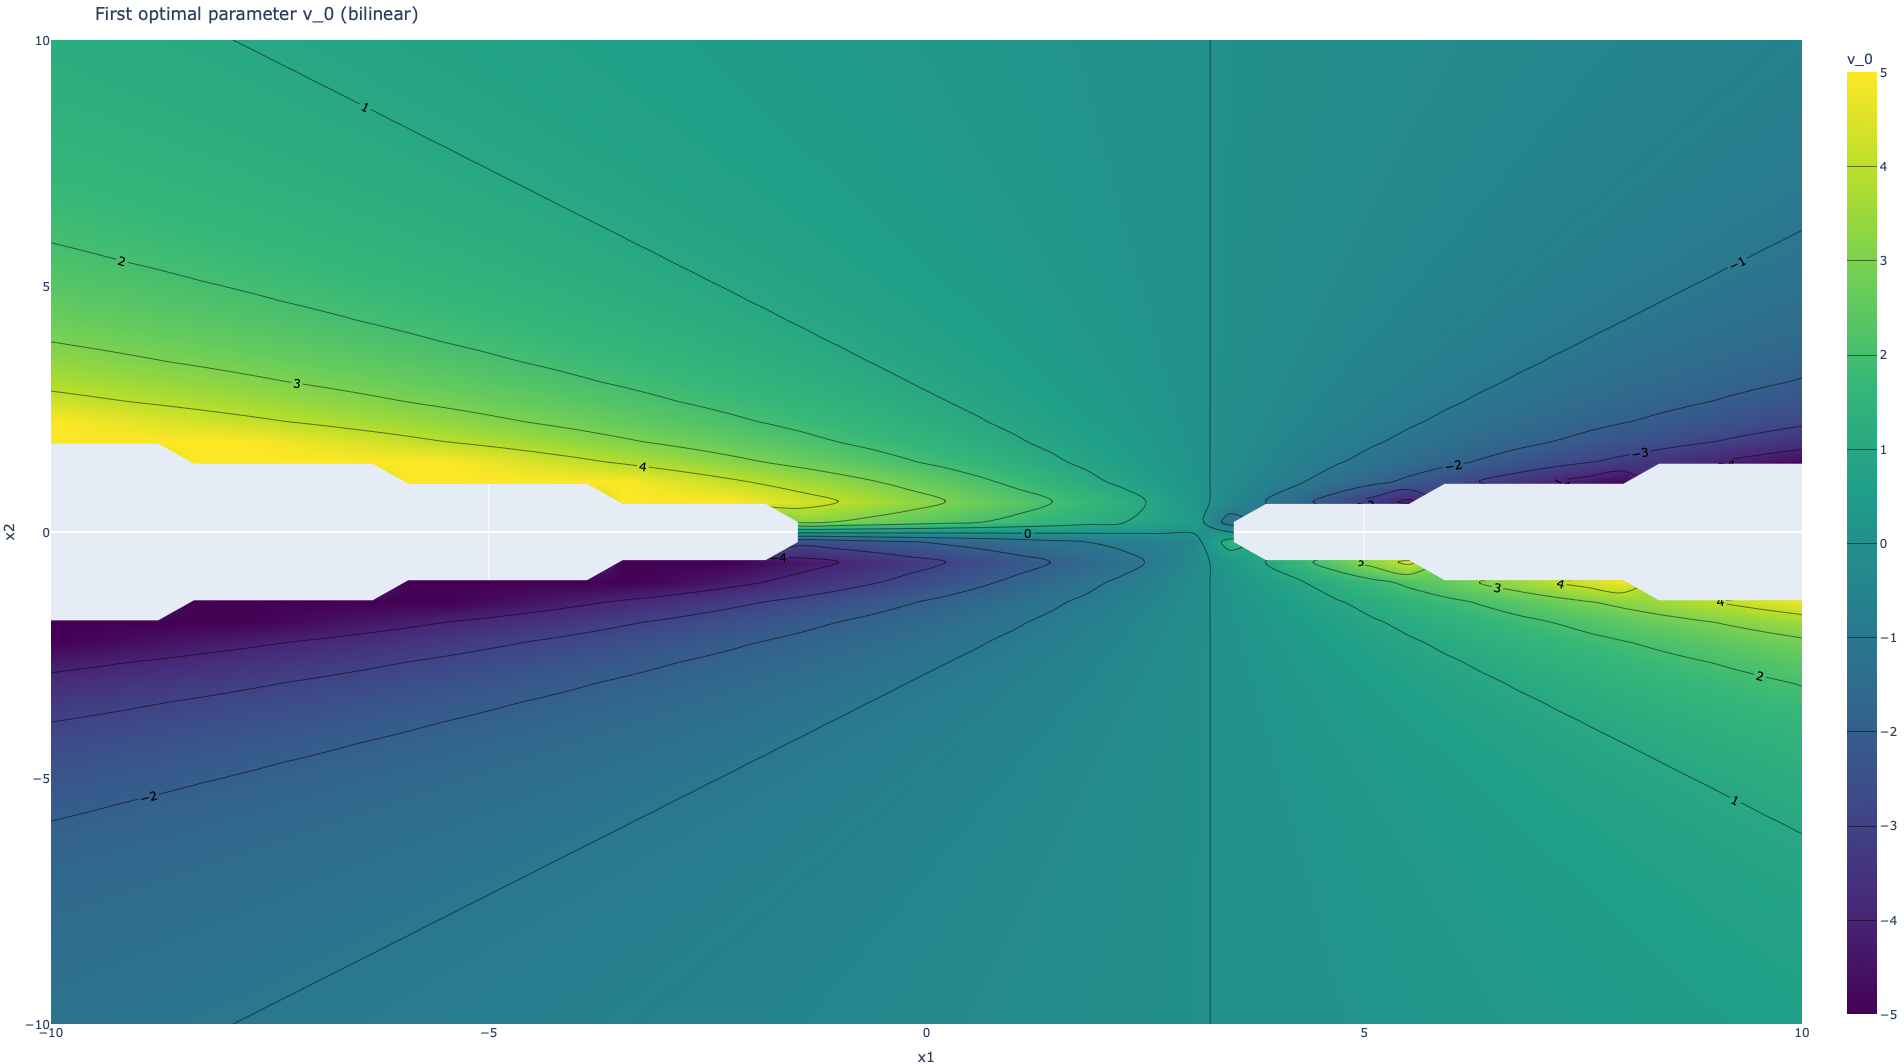
\includegraphics[width=\linewidth]{graphics/state_input_v_contour.png}
        \caption{Contour representation of \(v_0^\ast\) over the initial-state
        plane}
        \label{fig:state_input_v_contour}
    \end{minipage}
\end{figure}



The \(u_0^\ast\) surface shows how the immediate control action selected by
the optimizer depends on the initial values of \(x_1\) and \(x_2\). Similarly,
the \(v_0^\ast\) surface illustrates how the bilinear parameter is adjusted
depending on the state.

